
% ********** Chapter 9 **********
\chapter{Java ME Client}
\label{sec:JavaMEClient}

The Java ME Client is a client of web service interface which described in chapter \nolinebreak \ref{sec:WebServiceInterface}. It implemented all of the interfaces of web service of Web Call SDK. Besides the web service interface, Java ME Client also provide some convenient function such as load contact book from mobile phone and synchronize it with Web Call SDK server. 

\section{Architecture}
\label{sec:JavaMEClient:Architecture}

The architecture of Java ME web service client is shown in Figure \nolinebreak \ref{fig:TheArchitectureOfJavaMEClient}. It can be seen from the diagram that there are three layers in the Java ME client. They are, from bottom to top, Java ME API, Business Logic and User Interface. 

\begin{figure}[!hbtp]
\centering
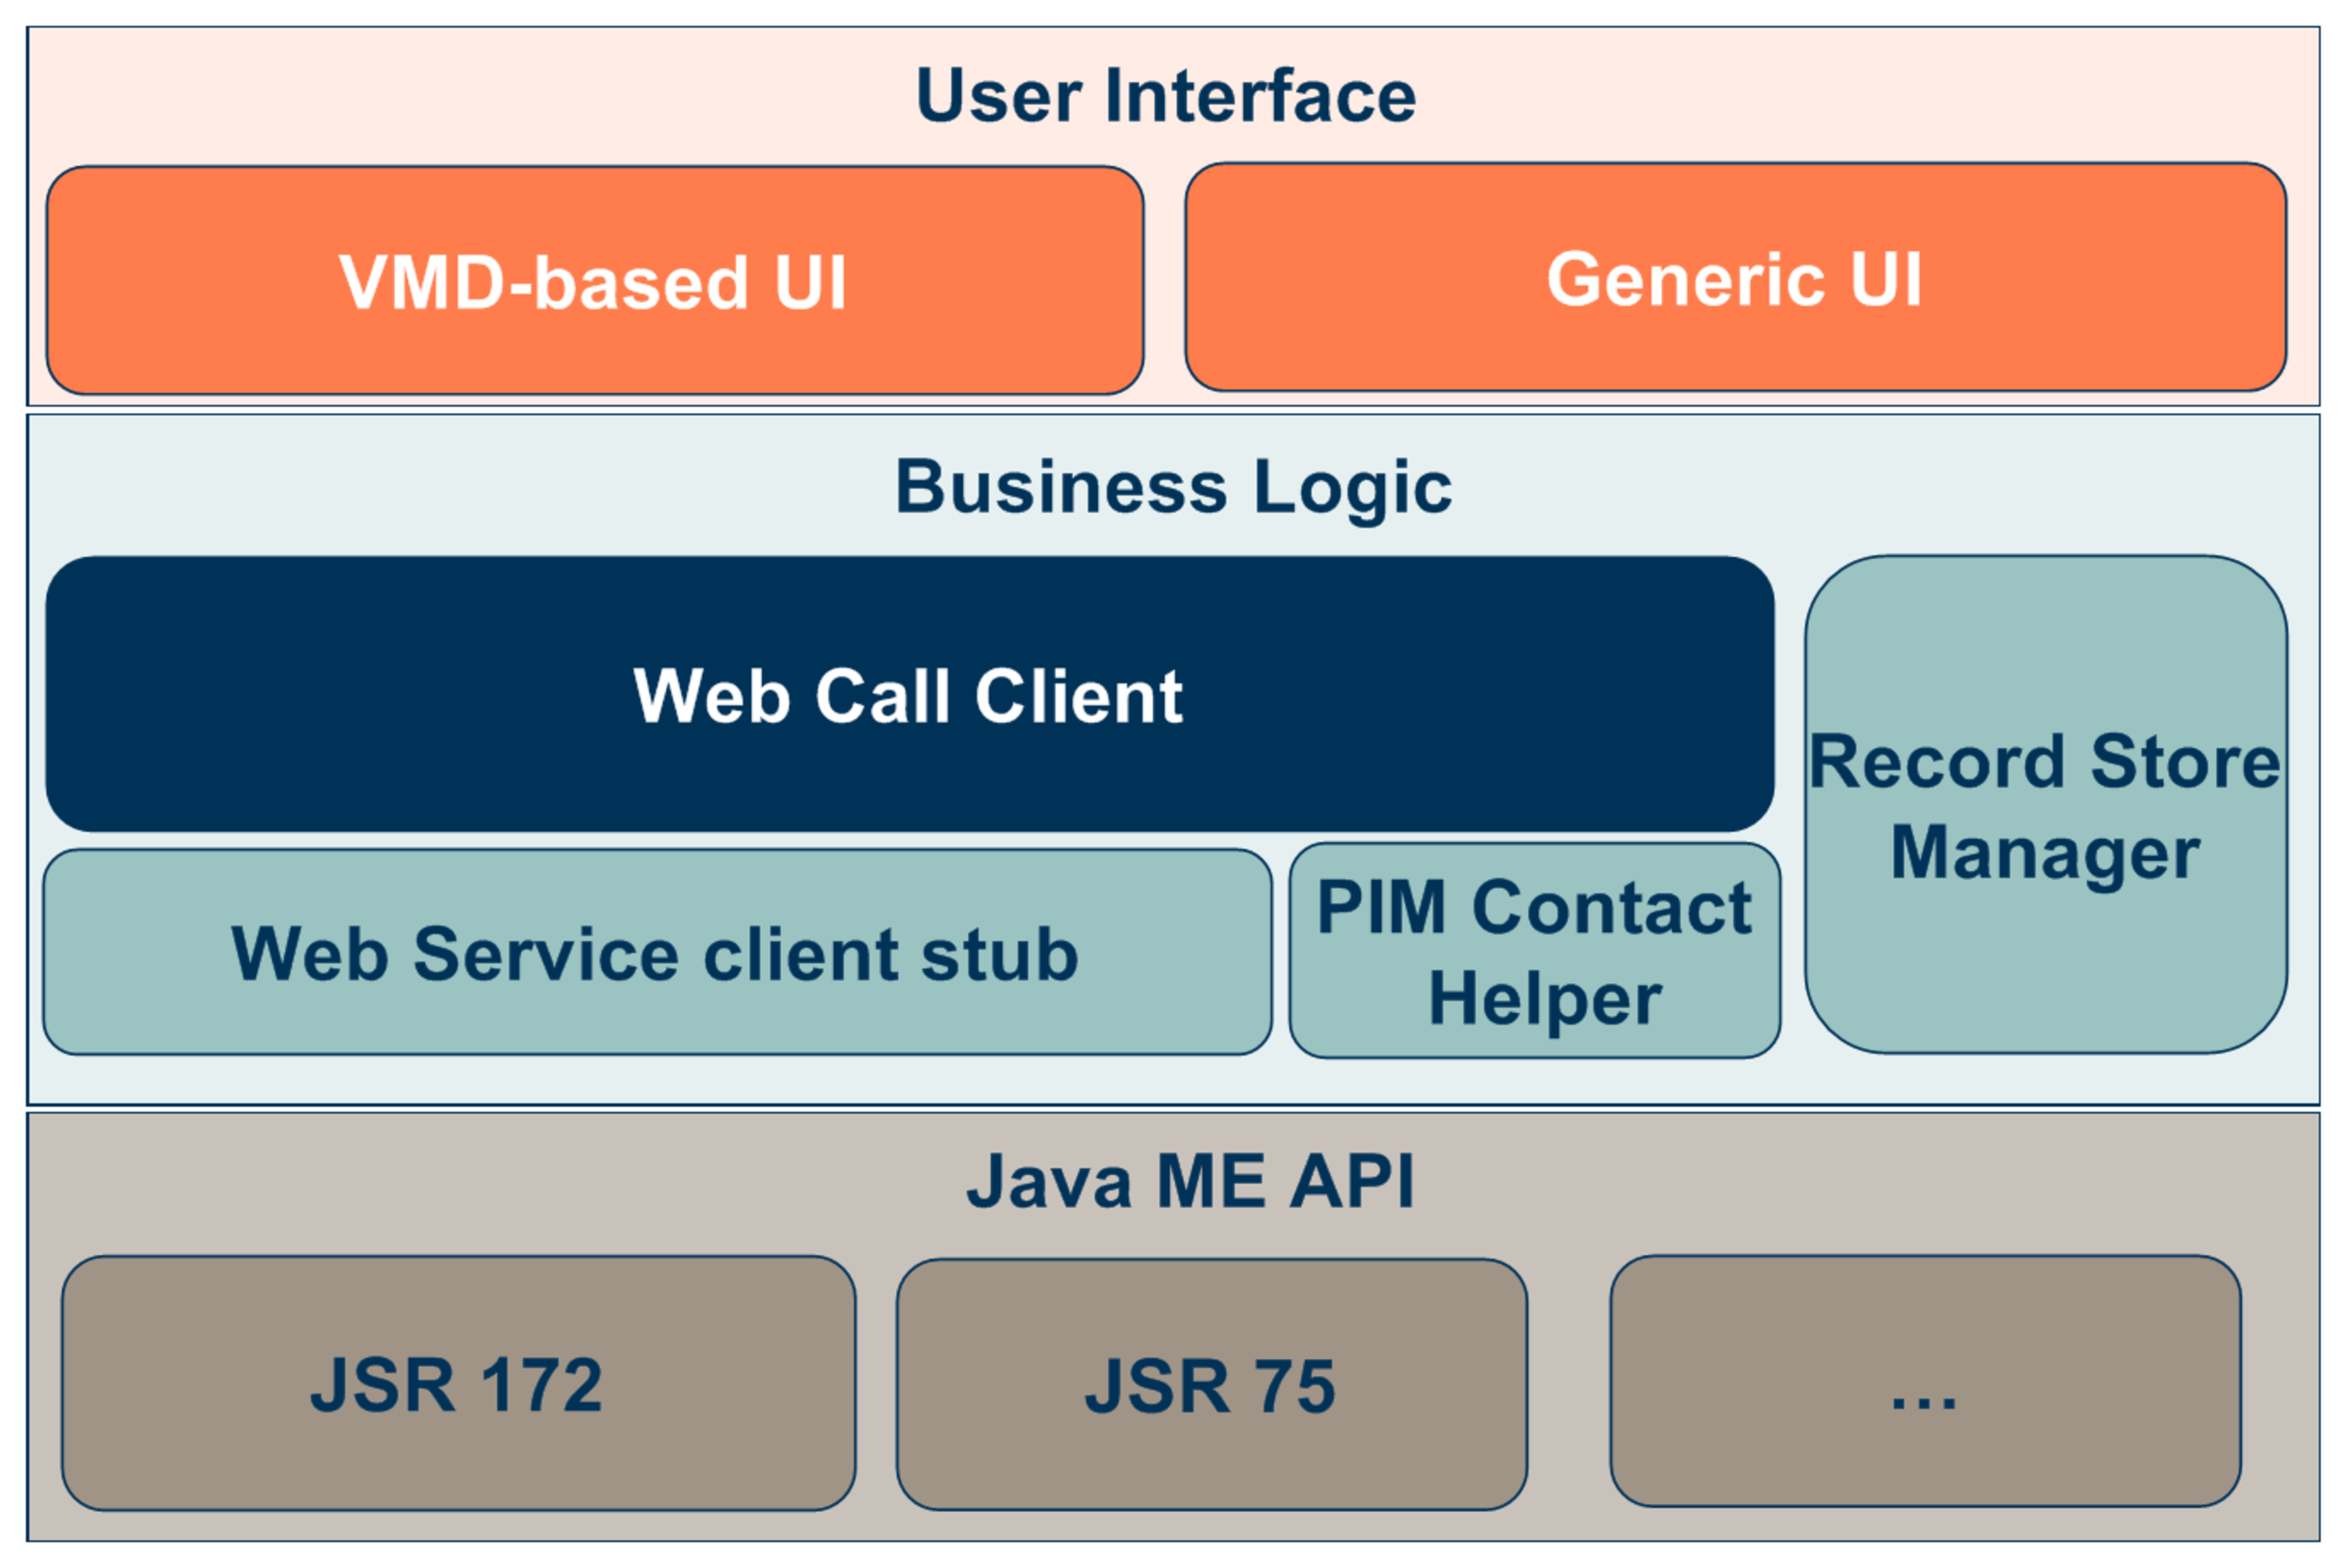
\epsfig{file=chap09/resources/java_me_client_architecture, width=5.2in}
\caption{The Architecture of Java ME Client}
\label{fig:TheArchitectureOfJavaMEClient}
\end{figure}

The Java ME API layer is the standard API set for Java ME platform. To meet the requirement of installation, the mobile device mast have a support of \texttt{JSR 172} (J2ME\texttrademark{} Web Services Specification)\cite{JSR172} and an optional support of \texttt{JSR 75} (PDA Optional Packages for the J2ME Platform)\cite{JSR75}. 

In business logic layer, there are several components that control the logic. A very important one, which is also the core of Java ME client, is the \texttt{Web Call Client}. The Web Call Client bases on \texttt{Web Call Client Stub} which is the client stub of web service interface of Web Call Example Application. The detail of Web Call Client and Web Service Client Stub will be discussed separately in section \ref{sec:JavaMEClient:WebCallClient} and \ref{sec:JavaMEClient:WebServiceClientStub}. The Web Call Client also uses a component named \texttt{Record Store Manager} which will be described in detail in section \ref{sec:JavaMEClient:RecordStoreManager}. The last component is \texttt{PIM Contact Helper}. It is a utility which helps to load contact book from mobile device.

In user interface (UI) layer, there are two implementation of UIs. The details of user interface will be shown in section \ref{sec:JavaMEClient:UserInterface}. 

\section{Web Service Client Stub}
\label{sec:JavaMEClient:WebServiceClientStub}

The web service client stub is a stub of web service interface which described in chapter \nolinebreak \ref{sec:WebServiceInterface}. It is generated by a wizard from NetBeans IDE. NetBeans is a open-source and free IDE sponsored by Sun Microsystems. The generation wizard is shown in Figure \ref{fig:NetbeansJavaMEWebServiceClientWizard}. The client stub is based on JSR 172, so only the handset which supports \texttt{JSR 172} can run the Java ME web service client.

\begin{figure}[!hbtp]
\centering
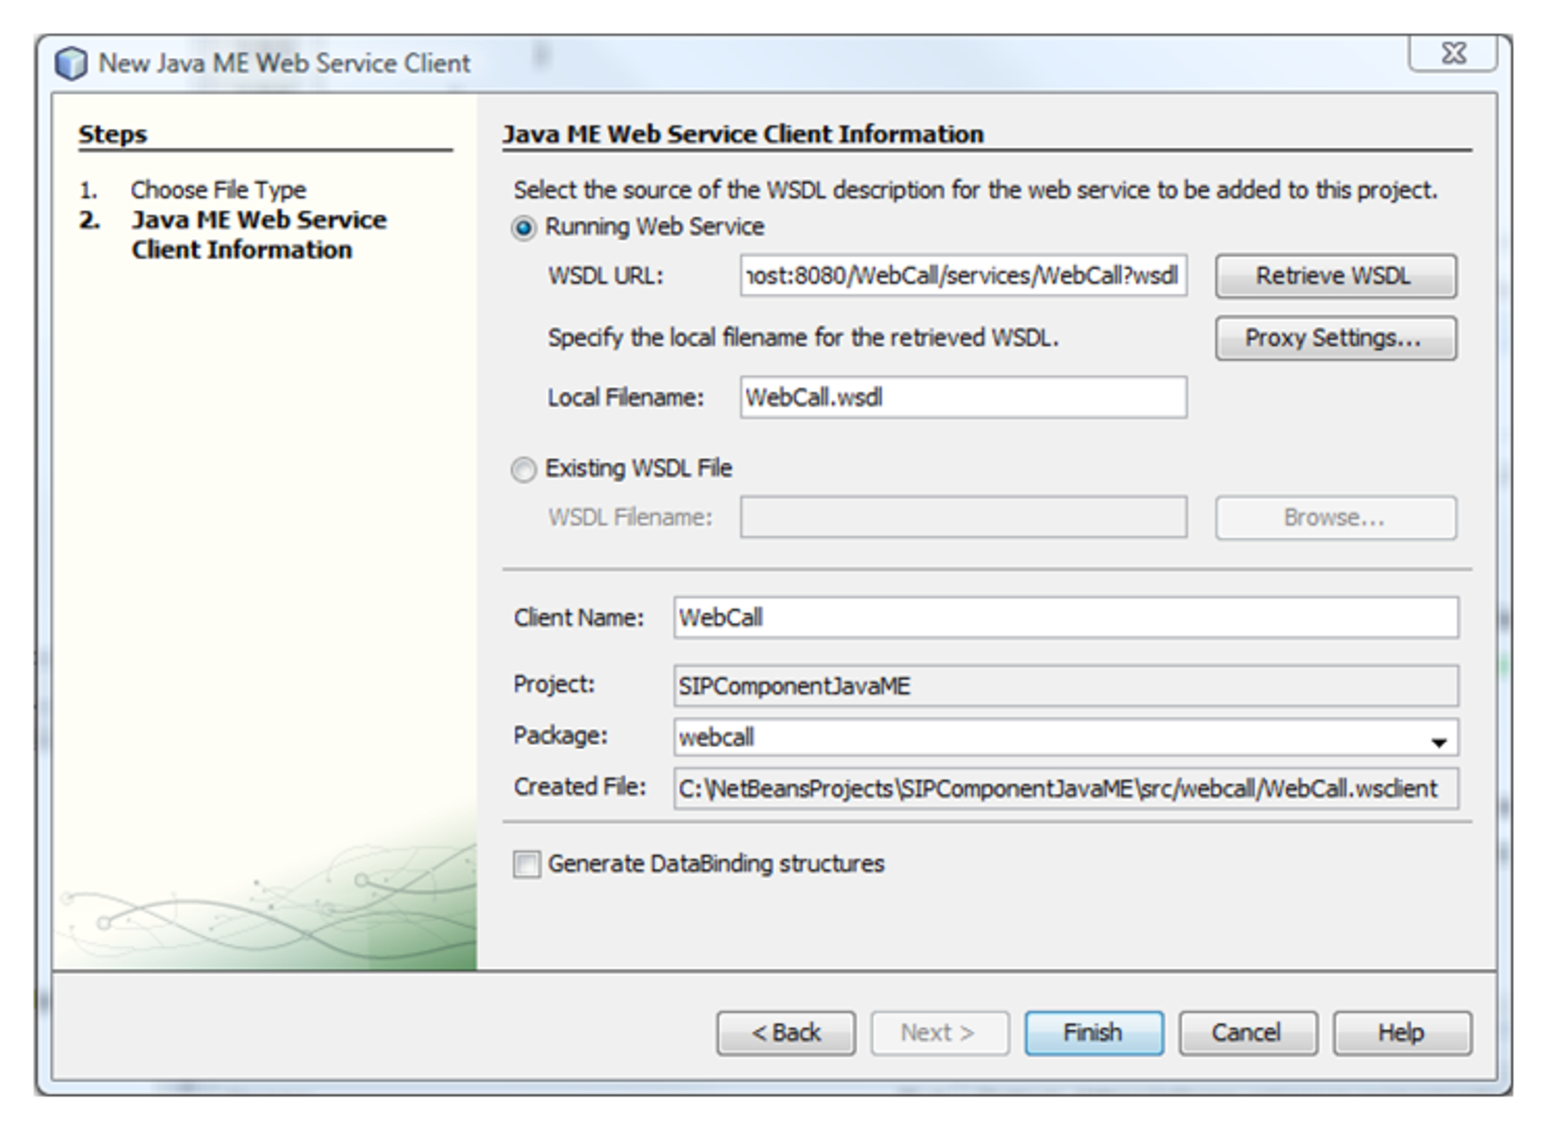
\epsfig{file=chap09/resources/Netbeans_Java_ME_Web_Service_Client_Wizard, width=5.2in}
\caption{Netbeans Java ME Web Service Client Wizard}
\label{fig:NetbeansJavaMEWebServiceClientWizard}
\end{figure}

Once the wizard is finished, NetBeans will automatically generate some classes that wrap the stub and make the operation of web service easily. And it communicates with web service server via SOAP protocol. The web service client stub is designed to be separately from the core logic of Java ME client (Web Service Client). This makes the lower stack of web service exchangeable. As just mentioned above, the client must be installed in a \texttt{JSR 172} enabler. The project team is planning to define a RESTful web service and a RESTful web service client to replace current SOAP based web service client stub. Since The RESTful web service only need a HTTP connection which is widely supported by modern mobile phones, the Java ME client will be installed on more devices by then. 


\section{Record Store Manager}
\label{sec:JavaMEClient:RecordStoreManager}

Record Store Manager is used for reading and writing the data from/to Java ME \textit{record management system} (RMS). It extends a abstract class which named \texttt{AbstractRecordStoreManager} which is a stand alone component which supplies a very convenient way to interactive with RMS. The \texttt{AbstractRecordStoreManager} wraps the action of saving and loading data to/from RMS. Two methods \texttt{setData()} and \texttt{getData()} handles everything. The \texttt{AbstractRecordStoreManager} can be not only used in Java ME Client of Web Call Example Application, but also other Java ME applications. A class hierarchy diagram of \texttt{RecordStoreManager} and \texttt{AbstractRecordStoreManager} is shown in Figure \ref{fig:TheClassDiagramofRecordStoreManager}.

\begin{figure}[!hbtp]
\centering
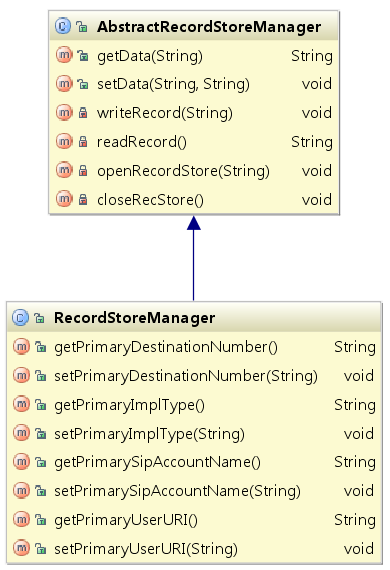
\epsfig{file=chap09/resources/record_store_manager, width=3in}
\caption{The Class Diagram of Record Store Manager}
\label{fig:TheClassDiagramofRecordStoreManager}
\end{figure}

\section{PIM Contact Helper}
\label{sec:JavaMEClient:PIMContactHelper}

\textsf{PIM Contact Helper} provides access to contact list of \textit{Personal Information Management} (PIM) data on J2ME devices. The PIM API is designed for a widely use and try to compatible with most of Java ME enabler. But it is lack of user friendly. The PIM Contact Helper wraps some APIs of JSR 75 and makes it very easy to load contact lists from mobile phone. Like \textsf{Record Store Manager}, \textsf{PIM Contact Helper} is also a stand alone component. It can also be used in other Java ME applications. To use it, the mobile device must support \texttt{JSR 75}\cite{JSR75}. When first the time use it, there will be pop up option window to ask if user want this application to read contacts list as shown in Figure \ref{fig:LoadPIMContacts}. As long as user approved, a phone contacts list will be shown on screen as shown in Figure \ref{fig:PIMContactsList}.  


\begin{figure}[!hbtp]
\centering
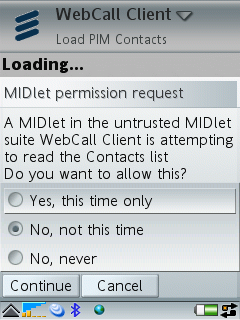
\epsfig{file=chap09/resources/load_pim_contacts, width=2.7in}
\caption{Load PIM Contacts}
\label{fig:LoadPIMContacts}
\end{figure}


\begin{figure}[!hbtp]
\centering
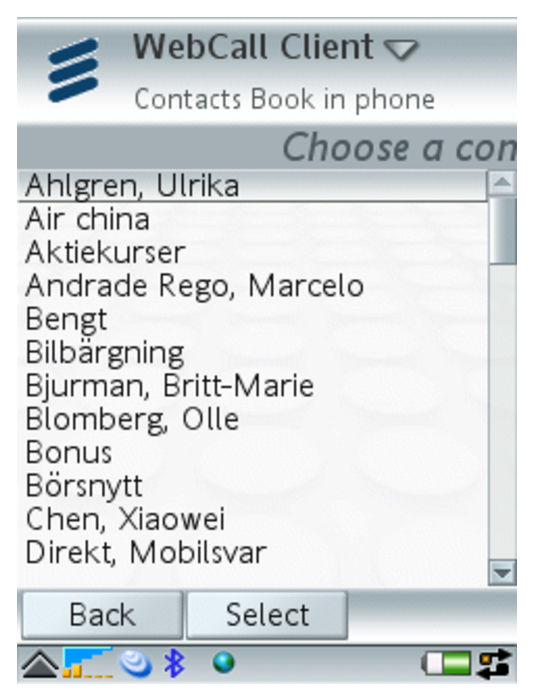
\epsfig{file=chap09/resources/pim_contacts, width=2.7in}
\caption{PIM Contacts List}
\label{fig:PIMContactsList}
\end{figure}

\section{Web Call Client}
\label{sec:JavaMEClient:WebCallClient}

The \textsf{Web Call Client} component bases on the \textsf{Web Service Client Stub}. As described in section \ref{sec:JavaMEClient:WebServiceClientStub}, The \textsf{Web Service Client Stub} implements only the client interface. And the \texttt{Web Call Client} manages the business logics, e.g. the load of last used configuration, the recent call list and logic of synchronization. The Web Call Client can be treated like a adapter between UI and Web Service Client Stub. It collects phone call information from UI and set them as parameters of Web Service Client Stub.

\section{User Interface}
\label{sec:JavaMEClient:UserInterface}

\subsection{VoIP Call Form}
\label{sec:JavaMEClient:UserInterface:VoIPCallForm}

A VoIP call form is shown in Figure \ref{fig:VoIPCallFormOfJavaMEClient}. On top of that form, there are two input fields, \textit{your phone number} and \textit{destination phone number}. Under that, where are two drop down lists. One is \textit{VoIP provider account}, and another is \textit{call method}. The contents of these two lists are fetched from web service interface. The VoIP provider is used to choose a VoIP account that user wishes to use. Users can also change the content of VoIP provider drop down lists via the desktop browser view or the mobile browser view. See how to configure the VoIP provider account, please refer to chapter \ref{sec:WebApplication}. Below that, there is a drop down list to choose call methods. There are five different methods to use. They have similar effects but not the same with of establishing connection. The differences of call method is talked in chapter \ref{sec:Solution}. A screen shot of call method drop down list is shown in Figure \ref{fig:CallMethodDropDownList}. The left bottom of this page is the ``Call'' button which will connect the phone call when use click it. Next to the call button is the ``Exit'' button.

\begin{figure}[!hbtp]
\centering
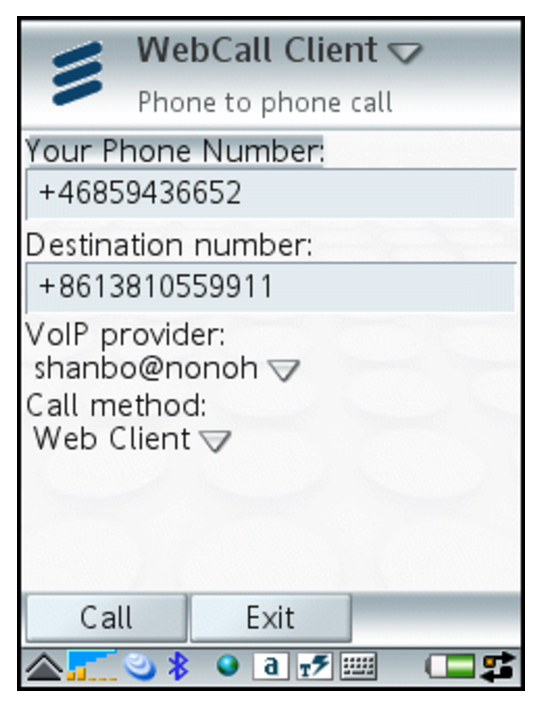
\epsfig{file=chap09/resources/VoIP_call_form, width=2.7in}
\caption{VoIP call form of Java ME Client}
\label{fig:VoIPCallFormOfJavaMEClient}
\end{figure}

\begin{figure}[!hbtp]
\centering
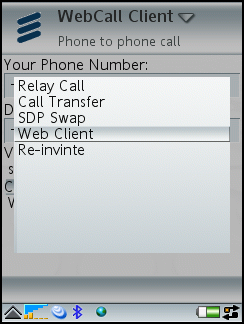
\epsfig{file=chap09/resources/call_method, width=2.7in}
\caption{Call method drop down list}
\label{fig:CallMethodDropDownList}
\end{figure}

The Java ME client use the RMS (Record Management System) to store the last call information include caller, callee, VoIP provider and call method. When the Java ME client starts again, it will read the record from RMS and automatically set call method as the same as last time used. The interaction with RMS is handled by \textsf{Record Store Manager} which is described in section \ref{sec:JavaMEClient:RecordStoreManager}.

On the VoIP call form menu, there are five screen menu items, PIM Contacts, My phone number, Contacts, Recent Call and Sync which is shown in in Figure \ref{fig:ScreenMenuItemsOfVoIPCallForm}. The functionalities of five menu items as well as phone call will be introduced within follow subsections.

\begin{figure}[!hbtp]
\centering
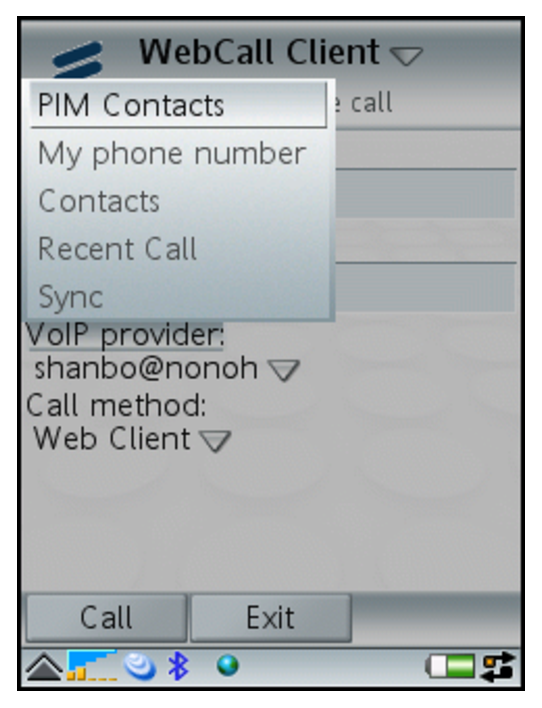
\epsfig{file=chap09/resources/VoIP_call_form_menu, width=2.7in}
\caption{Screen menu items of VoIP call form}
\label{fig:ScreenMenuItemsOfVoIPCallForm}
\end{figure}

\subsection{PIM Contacts}
\label{sec:JavaMEClient:UserInterface:PIMContacts}

PIM contacts supplies feature of reading contacts from Personal Information Management (PIM) data from cell phone. This function is implemented by the component of \textsf{PIM Contact Helper} which is described in section \ref{sec:JavaMEClient:PIMContactHelper}. In the view of ``Contacts Book in phone'' there is also another command to save your contacts in contact book of Java ME client. As long as user uses the synchronize function, the new contact will also be stored in the remote database of web application.

\subsection{My Phone Number}

My phone number is the phone number you wish to call from. It could your current phone or a landline phone. You can have more than one phone number saved in the database of server side. 
Click one of ``my phone number'', the number will be set as your phone number in the phone to phone call form.

\subsection{Contacts}

The contacts here refer to the contacts book in the web application. It is not same as the PIM contact list in phone memory. However, you can save contacts from contacts book in phone to contacts book in web application by the function mentioned in section \ref{sec:JavaMEClient:UserInterface:PIMContacts}. The number of selected contact will be set as destination number. The view of Contact list is shown in Figure \ref{fig:ContactListOfVoIPCallForm}.

\begin{figure}[!hbtp]
\centering
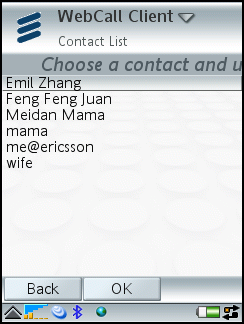
\epsfig{file=chap09/resources/contact_list, width=2.7in}
\caption{Contact list of VoIP call form}
\label{fig:ContactListOfVoIPCallForm}
\end{figure}

\subsection{Synchronize}

The synchronize function in phone call form is used to synchronize VoIP provider account and contacts. If same name with different phone number happens, the number in client will be kept. The synchronize function is shown in Figure \ref{fig:SynchronizeWithServer}.

\begin{figure}[!hbtp]
\centering
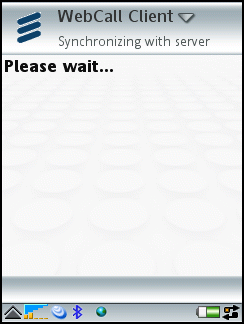
\epsfig{file=chap09/resources/synchronizing_with_server, width=2.7in}
\caption{Synchronize with server}
\label{fig:SynchronizeWithServer}
\end{figure}

\subsection{Phone Call}

After the user setup the phone number, destination number, VoIP provider account and Call method, just simply click ``Call'' button then a session will be established between the user and his friend.    

The phone call function in Java ME client is easy and convenient. Every time it restarts, the configuration will be the same as last time he used. It is especially useful when the user always calls the same number. The phone call function is shown in Figure \ref{fig:PhoneCallOfJavaMEClient}.

\begin{figure}[!hbtp]
\centering
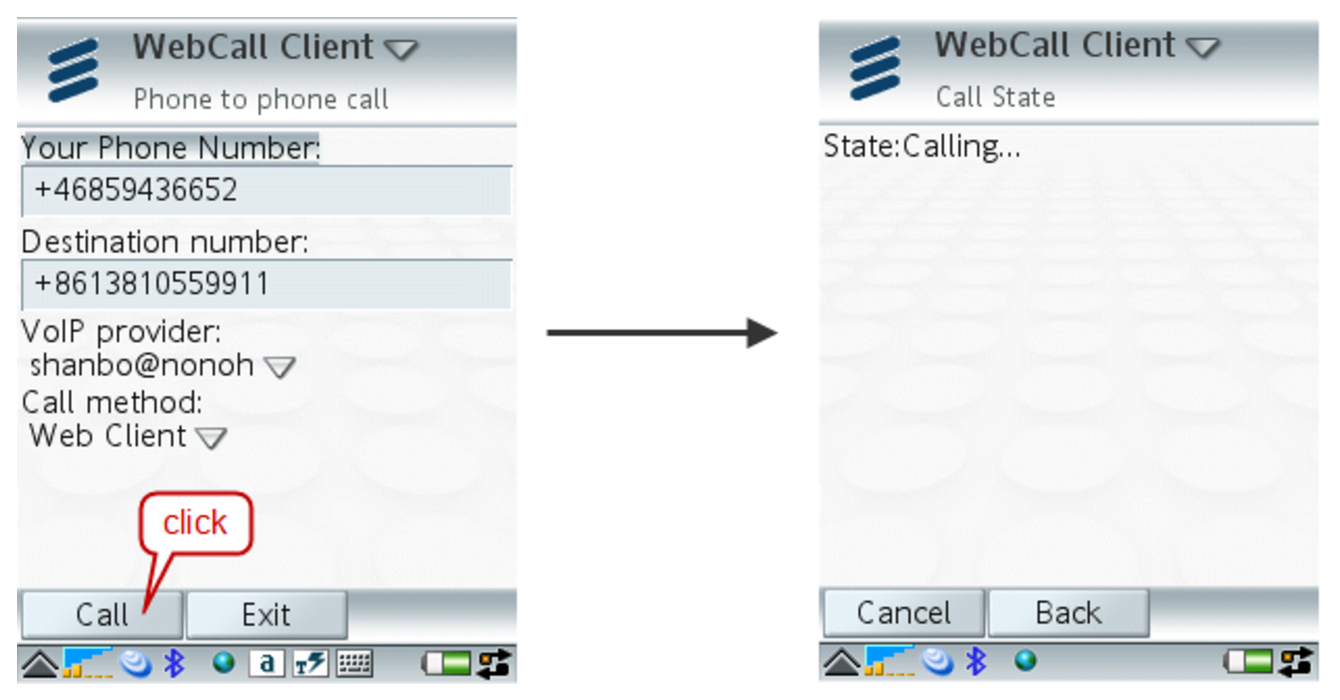
\epsfig{file=chap09/resources/VoIP_call, width=5.2in}
\caption{Phone call (via VoIP technology) of Java ME client}
\label{fig:PhoneCallOfJavaMEClient}
\end{figure}

\section{Two implementations of UI}

\subsection{VMD-based UI}
\label{sec:JavaMEClient:UserInterface:VMDBasedUI}

This Java ME client is first developed with Visual Mobile Designer. The Visual Mobile Designer (VMD) is a graphical interface within NetBeans Mobility that enables you to design mobile applications using drag and drop components. When compile and deploy the Java ME application, The application must include a NetBeans VMD library.

The VMD-based working flow is shown in Figure \ref{fig:JavaMEClientWorkingFlow}. For a larger image, please refer to the \textit{original version}\footnote{\url{http://shanbohomepage.googlecode.com/svn/trunk/master_thesis/chap09/resources/java_me_working_flow.png}} of working flow on web. 

\begin{figure}[!hbtp]
\centering
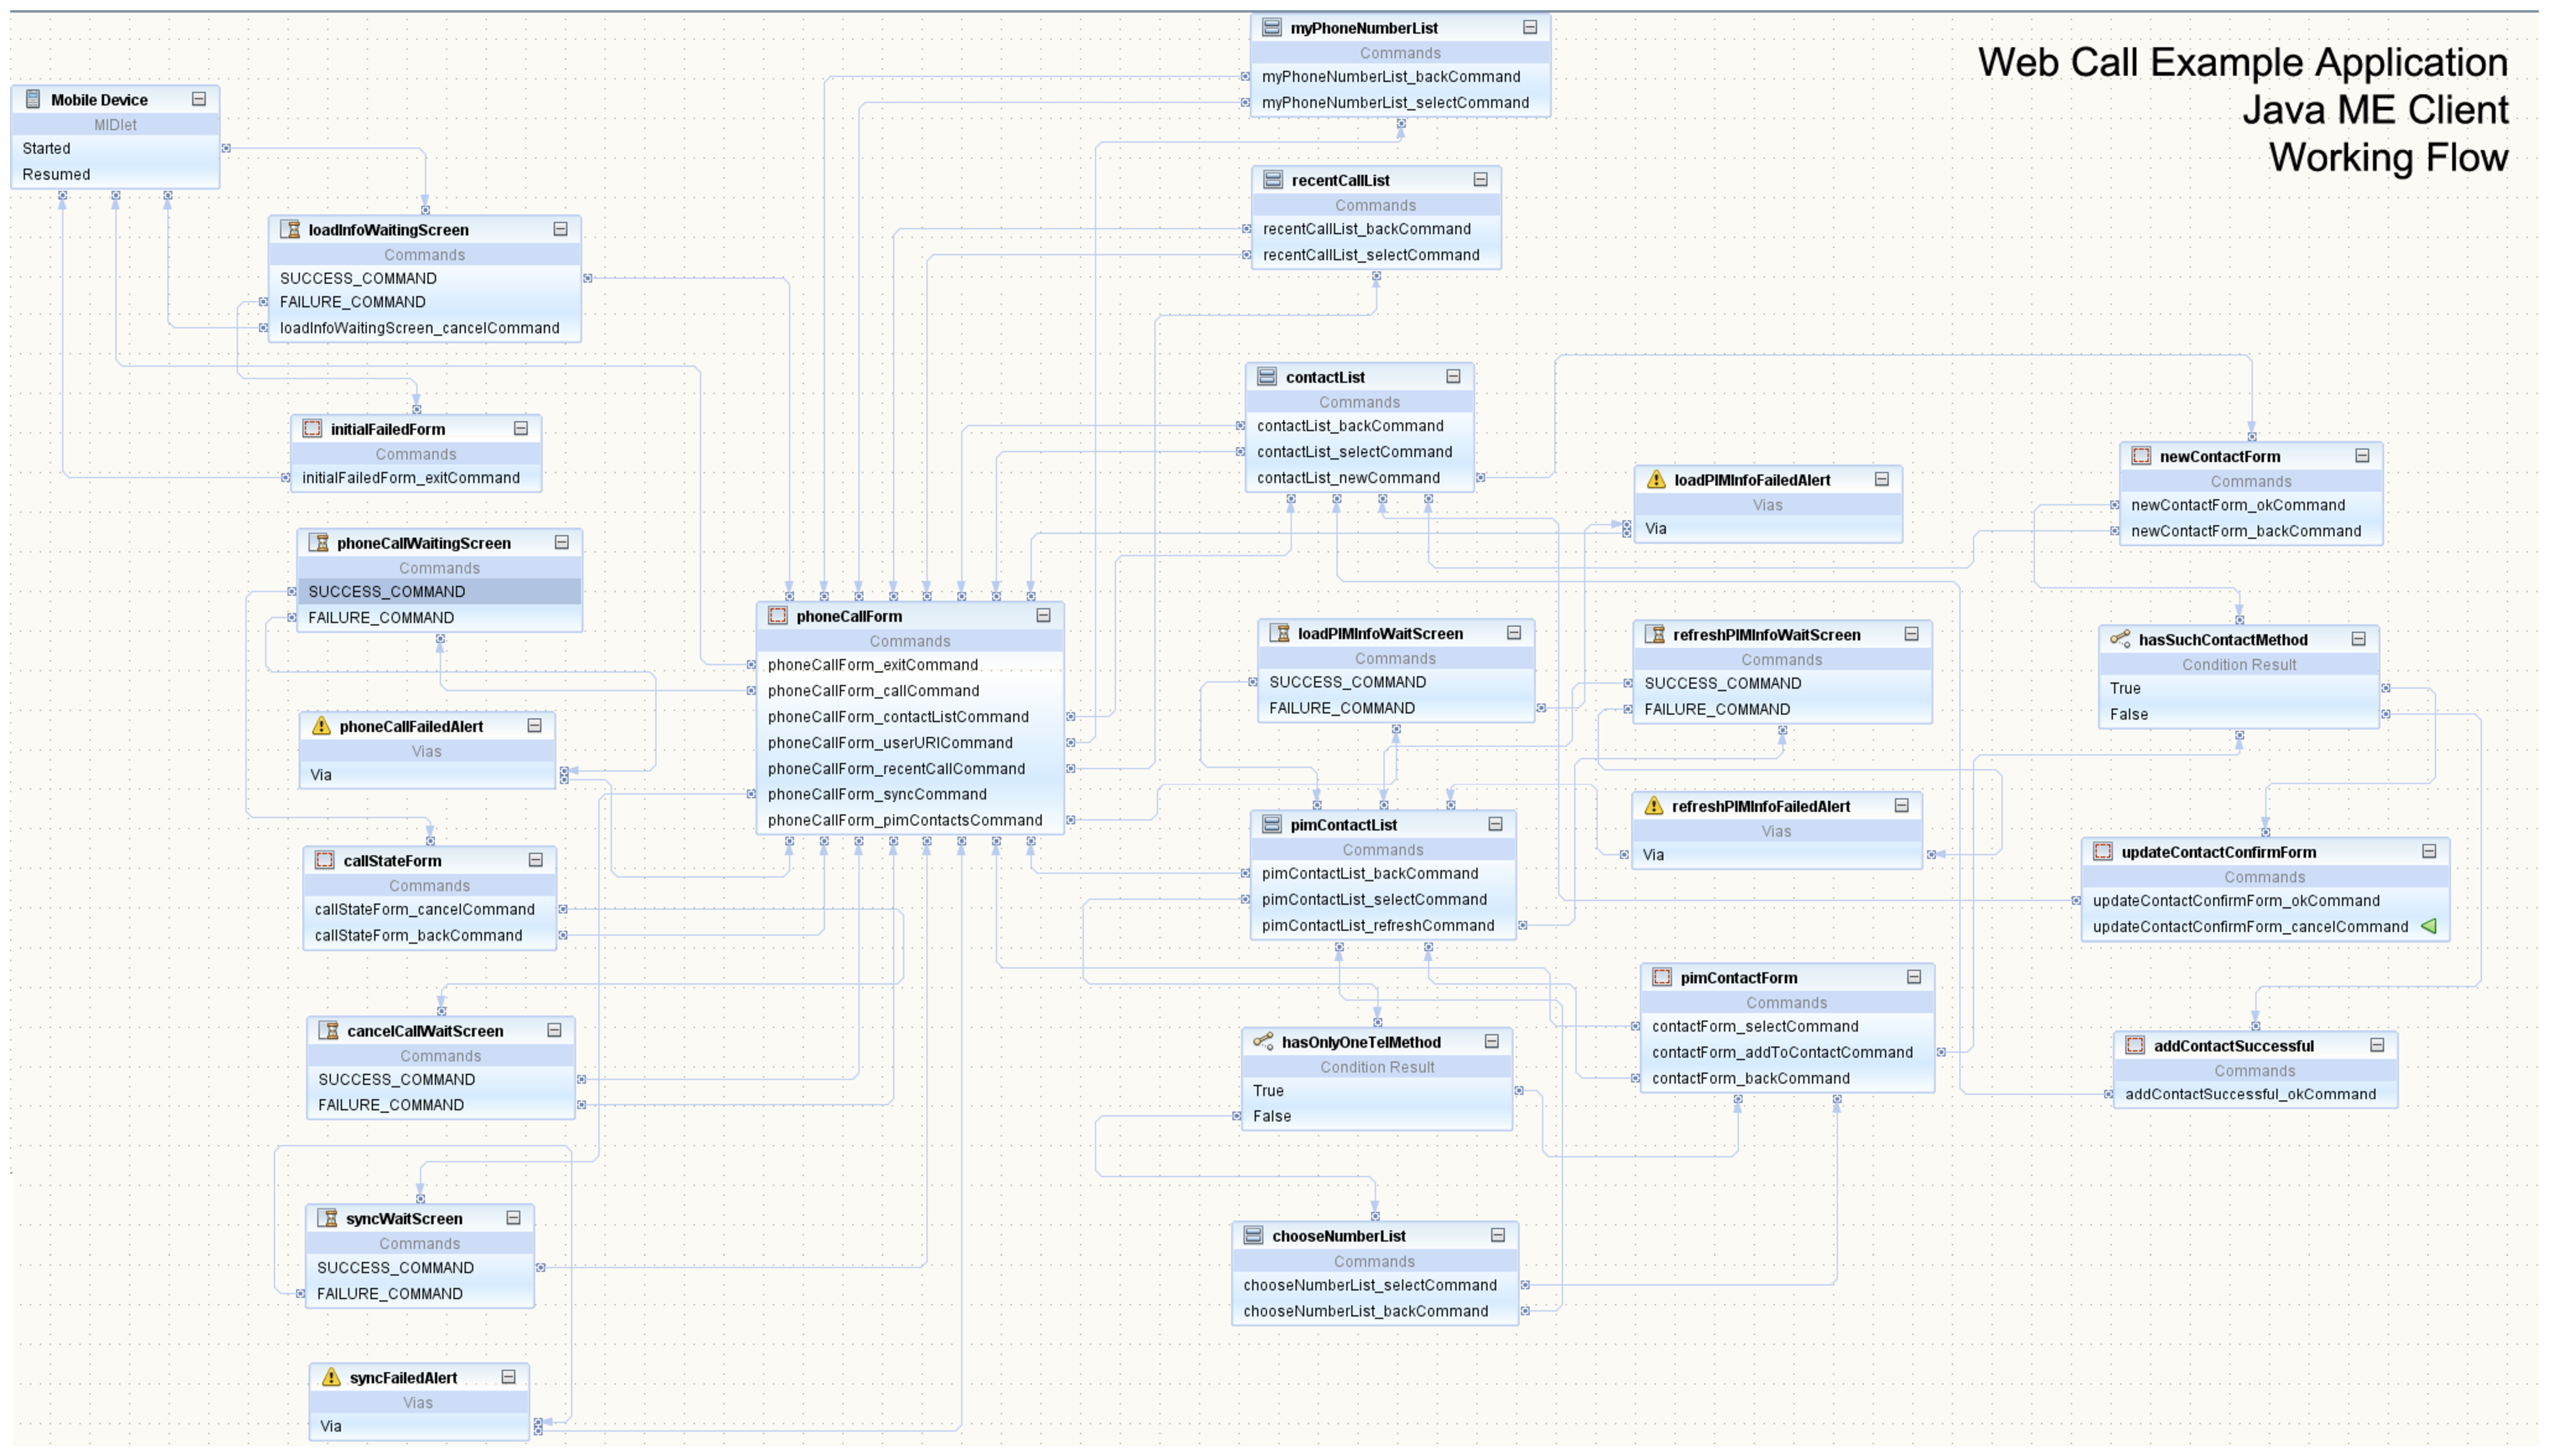
\epsfig{file=chap09/resources/java_me_working_flow, width=8.3in, angle=-90}
\caption{Java ME Client Working Flow}
\label{fig:JavaMEClientWorkingFlow}
\end{figure}


\subsection{Generic UI}
\label{sec:JavaMEClient:UserInterface:GenericUI}

To avoid using the VMD library, a generic UI is introduced. It doesn't use any particular class from NetBeans. Change \texttt{WaitScreen} to \texttt{Form}, change \\ \texttt{SimpleCancellableTask} to normal method. There are three sub packages in package \texttt{sip.components.me.ui}, \texttt{nb}, \texttt{nb2} and \texttt{general}. The package \texttt{nb} contains the VMD-based UI. The package \texttt{nb2} is a UI which doesn't contain any NetBeans library. The UI in package \texttt{general} is the code copy from nb2 and refractored according the package name and Midlet name. All three UIs can be treaded as Midlets.  They invoke the same logic in \textsf{Web Call Client} and \textsf{PIM Contact Helper}. By default only the UI in general will be compiled.

\section{Installation of Java ME Client}
\label{sec:JavaMEClient:InstallationOfJavaMEClient}

TODO: finish the text here

\section{Security of Java ME Client}
\label{sec:JavaMEClient:SecurityOfJavaMEClient}

TODO: finish the text here

% ********** End of chapter **********
